\documentclass[tikz,border=12pt]{standalone}
\usepackage{amsmath}
\usepackage{amssymb}
\usepackage{tikz}
\usetikzlibrary{calc,arrows.meta,decorations.pathmorphing,decorations.pathreplacing,positioning}

\begin{document}
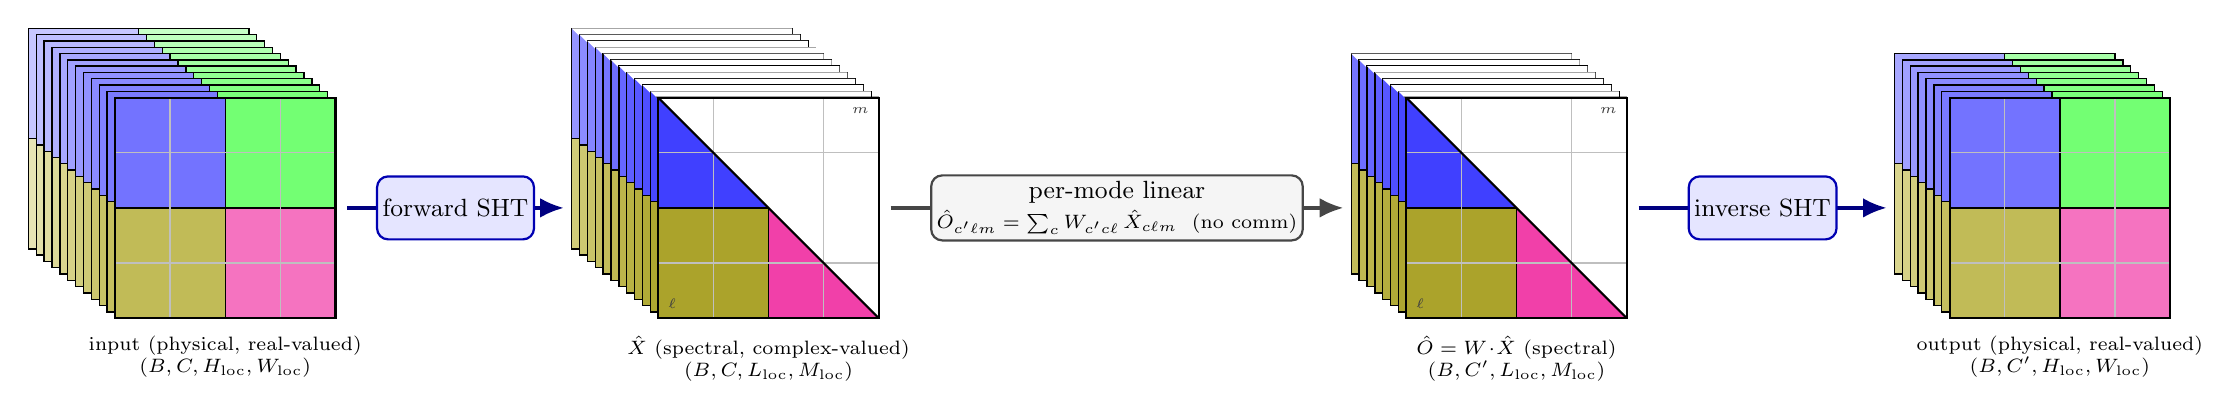
\begin{tikzpicture}[
  font=\sffamily,
  >=Latex,
  line width=0.5pt,
]

% ============================================================================
% Distributed Driscoll–Healy spectral convolution on S^2
%
%   x (physical, H×W sharded)
%     ── forward SHT (4 a2as) ──>   X̂ (spectral, L×M sharded)
%   per-mode linear   Ô[ℓ,m] = W[ℓ] · X̂[ℓ,m]   — fully local, no comm
%     ──>                          Ô (spectral, L×M sharded)
%     ── inverse SHT (4 a2as) ──>  y (physical, H×W sharded)
%
% The SHT internals (4 a2as each) are detailed in the SHT cartoon; this
% diagram treats them as black boxes so the central insight — that the
% mixing step is per-mode local — stands out.
% ============================================================================

% per-card stack offsets (channels go into the page, upper-left direction)
\def\dxIn{-0.10}\def\dyIn{0.08}

% ---------- helper: 2x2 yx-sharded grid (4 spatial ranks) ----------
\newcommand{\yxgrid}[4]{%
  \fill[blue!25!white,draw=black]    ({#1-#3},{#2})    rectangle ({#1},{#2+#3});
  \fill[green!30!white,draw=black]   ({#1},{#2})       rectangle ({#1+#3},{#2+#3});
  \fill[olive!30!white,draw=black]   ({#1-#3},{#2-#3}) rectangle ({#1},{#2});
  \fill[magenta!25!white,draw=black] ({#1},{#2-#3})    rectangle ({#1+#3},{#2});
  \foreach \i in {-1,1}{
    \draw[gray!50] ({#1+\i*#3/2},{#2-#3}) -- ({#1+\i*#3/2},{#2+#3});
    \draw[gray!50] ({#1-#3},{#2+\i*#3/2}) -- ({#1+#3},{#2+\i*#3/2});
  }
  \draw[thick] ({#1-#3},{#2-#3}) rectangle ({#1+#3},{#2+#3});
  \node[anchor=north,font=\scriptsize,align=center] at (#1,{#2-#3-0.10}) {#4};
}

% ---------- helper: stacked yx-grid (depth = channels) ----------
% args: cx, cy, halfwidth, n-cards, label
\newcommand{\yxstack}[5]{%
  \pgfmathtruncatemacro{\nm}{#4-1}%
  \foreach \k in {0,...,\nm}{%
    \pgfmathtruncatemacro{\j}{\nm-\k}%
    \pgfmathsetmacro{\ox}{#1 + \j*\dxIn}%
    \pgfmathsetmacro{\oy}{#2 + \j*\dyIn}%
    \pgfmathtruncatemacro{\sh}{55 - \j*3}%
    \fill[blue!\sh!white,draw=black]    ({\ox-#3},{\oy})    rectangle ({\ox},{\oy+#3});%
    \fill[green!\sh!white,draw=black]   ({\ox},{\oy})       rectangle ({\ox+#3},{\oy+#3});%
    \fill[olive!\sh!white,draw=black]   ({\ox-#3},{\oy-#3}) rectangle ({\ox},{\oy});%
    \fill[magenta!\sh!white,draw=black] ({\ox},{\oy-#3})    rectangle ({\ox+#3},{\oy});%
  }%
  \foreach \i in {-1,1}{
    \draw[gray!50] ({#1+\i*#3/2},{#2-#3}) -- ({#1+\i*#3/2},{#2+#3});
    \draw[gray!50] ({#1-#3},{#2+\i*#3/2}) -- ({#1+#3},{#2+\i*#3/2});
  }
  \draw[thick] ({#1-#3},{#2-#3}) rectangle ({#1+#3},{#2+#3});
  \node[anchor=north,font=\scriptsize,align=center] at (#1,{#2-#3-0.10}) {#5};
}

% ---------- helper: triangular L×M sharded spectral block ----------
\newcommand{\lmgrid}[4]{%
  \pgfmathsetmacro{\sx}{#1}\pgfmathsetmacro{\sy}{#2}\pgfmathsetmacro{\ss}{#3}
  \fill[blue!18!white,draw=black]    (\sx,         {\sy+\ss/2}) rectangle ({\sx+\ss/2}, {\sy+\ss});
  \fill[green!22!white,draw=black]   ({\sx+\ss/2}, {\sy+\ss/2}) rectangle ({\sx+\ss},   {\sy+\ss});
  \fill[olive!22!white,draw=black]   (\sx,         \sy)         rectangle ({\sx+\ss/2}, {\sy+\ss/2});
  \fill[magenta!18!white,draw=black] ({\sx+\ss/2}, \sy)         rectangle ({\sx+\ss},   {\sy+\ss/2});
  \foreach \i in {1,3}{
    \draw[gray!50] ({\sx+\i*\ss/4},\sy) -- ({\sx+\i*\ss/4},{\sy+\ss});
    \draw[gray!50] (\sx,{\sy+\i*\ss/4}) -- ({\sx+\ss},{\sy+\i*\ss/4});
  }
  \draw[thick] (\sx,\sy) rectangle ({\sx+\ss},{\sy+\ss});
  \fill[white] ({\sx+\ss},{\sy+\ss}) -- (\sx,{\sy+\ss}) -- ({\sx+\ss},\sy) -- cycle;
  \draw[thick] ({\sx+\ss},{\sy+\ss}) -- (\sx,{\sy+\ss}) -- ({\sx+\ss},\sy);
  \node[font=\tiny,anchor=south west,gray!50!black] at (\sx,\sy) {$\ell$};
  \node[font=\tiny,anchor=north east,gray!50!black] at ({\sx+\ss},{\sy+\ss}) {$m$};
  \node[anchor=north,font=\scriptsize,align=center] at ({\sx+\ss/2},{\sy-0.10}) {#4};
}

% ---------- helper: stacked lmgrid (channels = card stack on the L×M triangle) ----
% args: lower-left x, lower-left y, side, n-cards, front-saturation, label
\newcommand{\lmstack}[6]{%
  \pgfmathtruncatemacro{\nm}{#4-1}%
  \foreach \k in {0,...,\nm}{%
    \pgfmathtruncatemacro{\j}{\nm-\k}%
    \pgfmathsetmacro{\sx}{#1 + \j*\dxIn}%
    \pgfmathsetmacro{\sy}{#2 + \j*\dyIn}%
    \pgfmathsetmacro{\ss}{#3}%
    \pgfmathtruncatemacro{\sh}{#5 - \j*3}%
    \fill[blue!\sh!white,draw=black]    (\sx,         {\sy+\ss/2}) rectangle ({\sx+\ss/2}, {\sy+\ss});%
    \fill[green!\sh!white,draw=black]   ({\sx+\ss/2}, {\sy+\ss/2}) rectangle ({\sx+\ss},   {\sy+\ss});%
    \fill[olive!\sh!white,draw=black]   (\sx,         \sy)         rectangle ({\sx+\ss/2}, {\sy+\ss/2});%
    \fill[magenta!\sh!white,draw=black] ({\sx+\ss/2}, \sy)         rectangle ({\sx+\ss},   {\sy+\ss/2});%
    \fill[white] ({\sx+\ss},{\sy+\ss}) -- (\sx,{\sy+\ss}) -- ({\sx+\ss},\sy) -- cycle;%
  }%
  \foreach \i in {1,3}{
    \draw[gray!50] ({#1+\i*#3/4},#2) -- ({#1+\i*#3/4},{#2+#3});
    \draw[gray!50] (#1,{#2+\i*#3/4}) -- ({#1+#3},{#2+\i*#3/4});
  }
  \draw[thick] (#1,#2) rectangle ({#1+#3},{#2+#3});
  \draw[thick] ({#1+#3},{#2+#3}) -- (#1,{#2+#3}) -- ({#1+#3},#2);
  \node[font=\tiny,anchor=south west,gray!50!black] at (#1,#2) {$\ell$};
  \node[font=\tiny,anchor=north east,gray!50!black] at ({#1+#3},{#2+#3}) {$m$};
  \node[anchor=north,font=\scriptsize,align=center] at ({#1+#3/2},{#2-0.10}) {#6};
}

% ============================================================================
% LAYOUT — four blocks horizontally
%
%   [physical input] ─SHT(4 a2as)─▶ [spectral X̂] ─local mix─▶ [spectral Ô] ─iSHT(4 a2as)─▶ [physical output]
% ============================================================================

% common geometry
\def\gH{1.4}       % yxstack half-width
\def\sH{2.8}       % lmstack side
% baseline for the grids: align their centres on y = 0
\def\yYx{0}        % yxstack centre y
\def\ySpec{-1.4}   % lmstack lower-left y (so its centre also sits at 0)
\def\arrowY{0}     % arrow baseline (close to the visual centre of both stack sizes)

% channel-stack depths — C ≠ C', so the two halves of the cartoon use
% different N. The "fan" of cards behind each block reads as the channel
% dimension at a glance.
\def\Nin{12}       % input/X̂ channel cards   (= C)
\def\Nout{8}       % Ô/output channel cards   (= C')

% --------- B1: physical input ---------
\def\xIn{0}
\yxstack{\xIn}{\yYx}{\gH}{\Nin}{input (physical, real-valued)\\$(B,C,H_\text{loc},W_\text{loc})$};

% --------- B2: spectral coefficients (after forward SHT) ---------
\def\xXh{5.5}
\lmstack{\xXh}{\ySpec}{\sH}{\Nin}{75}{$\hat{X}$ (spectral, complex-valued)\\$(B,C,L_\text{loc},M_\text{loc})$};

% --------- B3: spectral coefficients (after per-mode mixing) ---------
% Stack thins from \Nin → \Nout to reflect C → C'.
\def\xYh{15.0}
\lmstack{\xYh}{\ySpec}{\sH}{\Nout}{75}{$\hat{O}=W\!\cdot\!\hat{X}$ (spectral)\\$(B,C',L_\text{loc},M_\text{loc})$};

% --------- B4: physical output (after inverse SHT) ---------
\def\xOut{23.3}
\yxstack{\xOut}{\yYx}{\gH}{\Nout}{output (physical, real-valued)\\$(B,C',H_\text{loc},W_\text{loc})$};

% ============================================================================
% ARROWS
% ============================================================================

% Back-card depth offset for each stack — \dxIn is negative, so the
% back-most card sits this far to the LEFT of the front card's anchor.
\pgfmathsetmacro{\dInBack}{-(\Nin-1)*\dxIn}      % = 1.1 for \Nin=12
\pgfmathsetmacro{\dOutBack}{-(\Nout-1)*\dxIn}    % = 0.7 for \Nout=8

% --- A1: input → X̂ (forward SHT, 4 a2as bundled into a box) ---
% Arrow lands at the back-card left edge of B2's lmstack (xXh - dInBack).
\coordinate (a1s) at ({\xIn+\gH+0.15},\arrowY);
\coordinate (a1e) at ({\xXh-\dInBack-0.10},\arrowY);
\draw[-{Latex[length=3mm,width=2.5mm]},very thick,blue!50!black] (a1s) -- (a1e);
\node[draw=blue!70!black,thick,fill=blue!10,rounded corners,
      minimum width=18mm,minimum height=8mm,align=center,font=\small,inner sep=2pt]
  (sht1) at ($(a1s)!0.5!(a1e)$) {forward SHT};

% --- A2: X̂ → Ô (per-mode linear — fully local, no comm) ---
\coordinate (a2s) at ({\xXh+\sH+0.15},\arrowY);
\coordinate (a2e) at ({\xYh-\dOutBack-0.10},\arrowY);
\draw[-{Latex[length=3mm,width=2.5mm]},very thick,gray!55!black] (a2s) -- (a2e);
\node[draw=gray!55!black,thick,fill=gray!8,rounded corners,
      minimum width=22mm,minimum height=8mm,align=center,font=\small,inner sep=2pt]
  (mix) at ($(a2s)!0.5!(a2e)$)
  {per-mode linear\\{\scriptsize $\hat{O}_{c'\ell m}=\sum_c W_{c'c\ell}\,\hat{X}_{c\ell m}$\,\, (no comm)}};

% --- A3: Ô → output (inverse SHT, 4 a2as) ---
% B4 yxstack: back-card left edge at xOut - gH - dOutBack.
\coordinate (a3s) at ({\xYh+\sH+0.15},\arrowY);
\coordinate (a3e) at ({\xOut-\gH-\dOutBack-0.10},\arrowY);
\draw[-{Latex[length=3mm,width=2.5mm]},very thick,blue!50!black] (a3s) -- (a3e);
\node[draw=blue!70!black,thick,fill=blue!10,rounded corners,
      minimum width=18mm,minimum height=8mm,align=center,font=\small,inner sep=2pt]
  (sht2) at ($(a3s)!0.5!(a3e)$) {inverse SHT};

% ============================================================================
% Top annotation (optional — uncomment for a title)
% ============================================================================
%\node[font=\large\bfseries,anchor=south,gray!25!black]
%  at ({(\xIn+\xOut)/2}, 2.4)
%  {Distributed DH spectral convolution on $S^2$};
%
%\node[font=\scriptsize,anchor=south,align=center,gray!45!black,text width=14cm]
%  at ({(\xIn+\xOut)/2}, 2.0)
%  {\textit{Communication is confined to the two SHTs; the spectral mixing is per-mode local.}};

\end{tikzpicture}
\end{document}
